
\section{Ergebnisse}
Wir haben unsere Generative Adversial Networks nun zur Generierung von Plattformen, Schweinen, TNTs und Blöcke eingesetzt. Dabei stellen wir für die verschiedenen Gegenstände fest, dass unterschiedliche Ergebnisse erzielt wurden. Im ersten Fall widmen wir uns den Plattformen. Bei diesen fällt auf, dass aus dem Ursprungsbild Konturen herausstechen und eine Form annehmen. In unserem Beispiel haben wir knapp sechs Tausend, sich immer weiter verbessernde Bilder generieren lassen. Auffällig dabei ist jedoch, dass die Konturen und Formen, die Plattformen darstellen sollen, immer flächenartiger werden und somit eine geeignete Grundlage darstellen sollten, diese allerdings in ihrer Struktur sinnfrei und zum Teil identisch mit einem vollständig flachen Level ist. Es sind weder Plattformen in der Höhe bzw. außergewöhnliche Formen aufzufinden, welche den Spielspaß verbessern könnten. \\ Anders sieht es hier bei den punktförmigen Gegenständen, wie den Schweinen und TNTs, aus. Diese können mithilfe des GAN bisher gut innerhalb des Levels verstreut werden. Es kommt weiterhin vor, dass Schweine sehr nah beieinander stehen und deshalb in den GAN als eine Linie generiert werden (si. Verdeutlichen der Konturen der erzeugten RAW-Bilder zur besseren Erkennung von Training). \\Leider besteht auch hier das Problem, dass Faktoren wie Spaß und Herausforderung (bisher) nicht eingebracht werden konnten, weswegen die Verteilung der einzelnen Objekte derzeit willkürlich ausfällt. Dieses Problem zieht sich auch durch die anderen Gegenstände. \\ \\Ein weiteres Problem stellt die Verteilung der punktförmigen Gegenstände dar. Am Beispiel der Schweine fällt diese auf den Blick zwar sinnvoll aus, da diese passend über das Level verstreut oder nachvollziehbar angeordnet sind. Nur häufig finden sich keine Blöcke unter den Gegenständen, sodass diese beim Start des Levels durch das Fallen entweder zwingend ihren Standort verändern oder sogar ohne Einwirkung des Spielers sofort sterben. Dies ist jedoch fatal für das Spielprinzip, da die Schweine nur durch die Aktionen des Spielers zu eliminieren sein sollten (vgl. Abbildung 3).
\begin{figure}
	\centering
	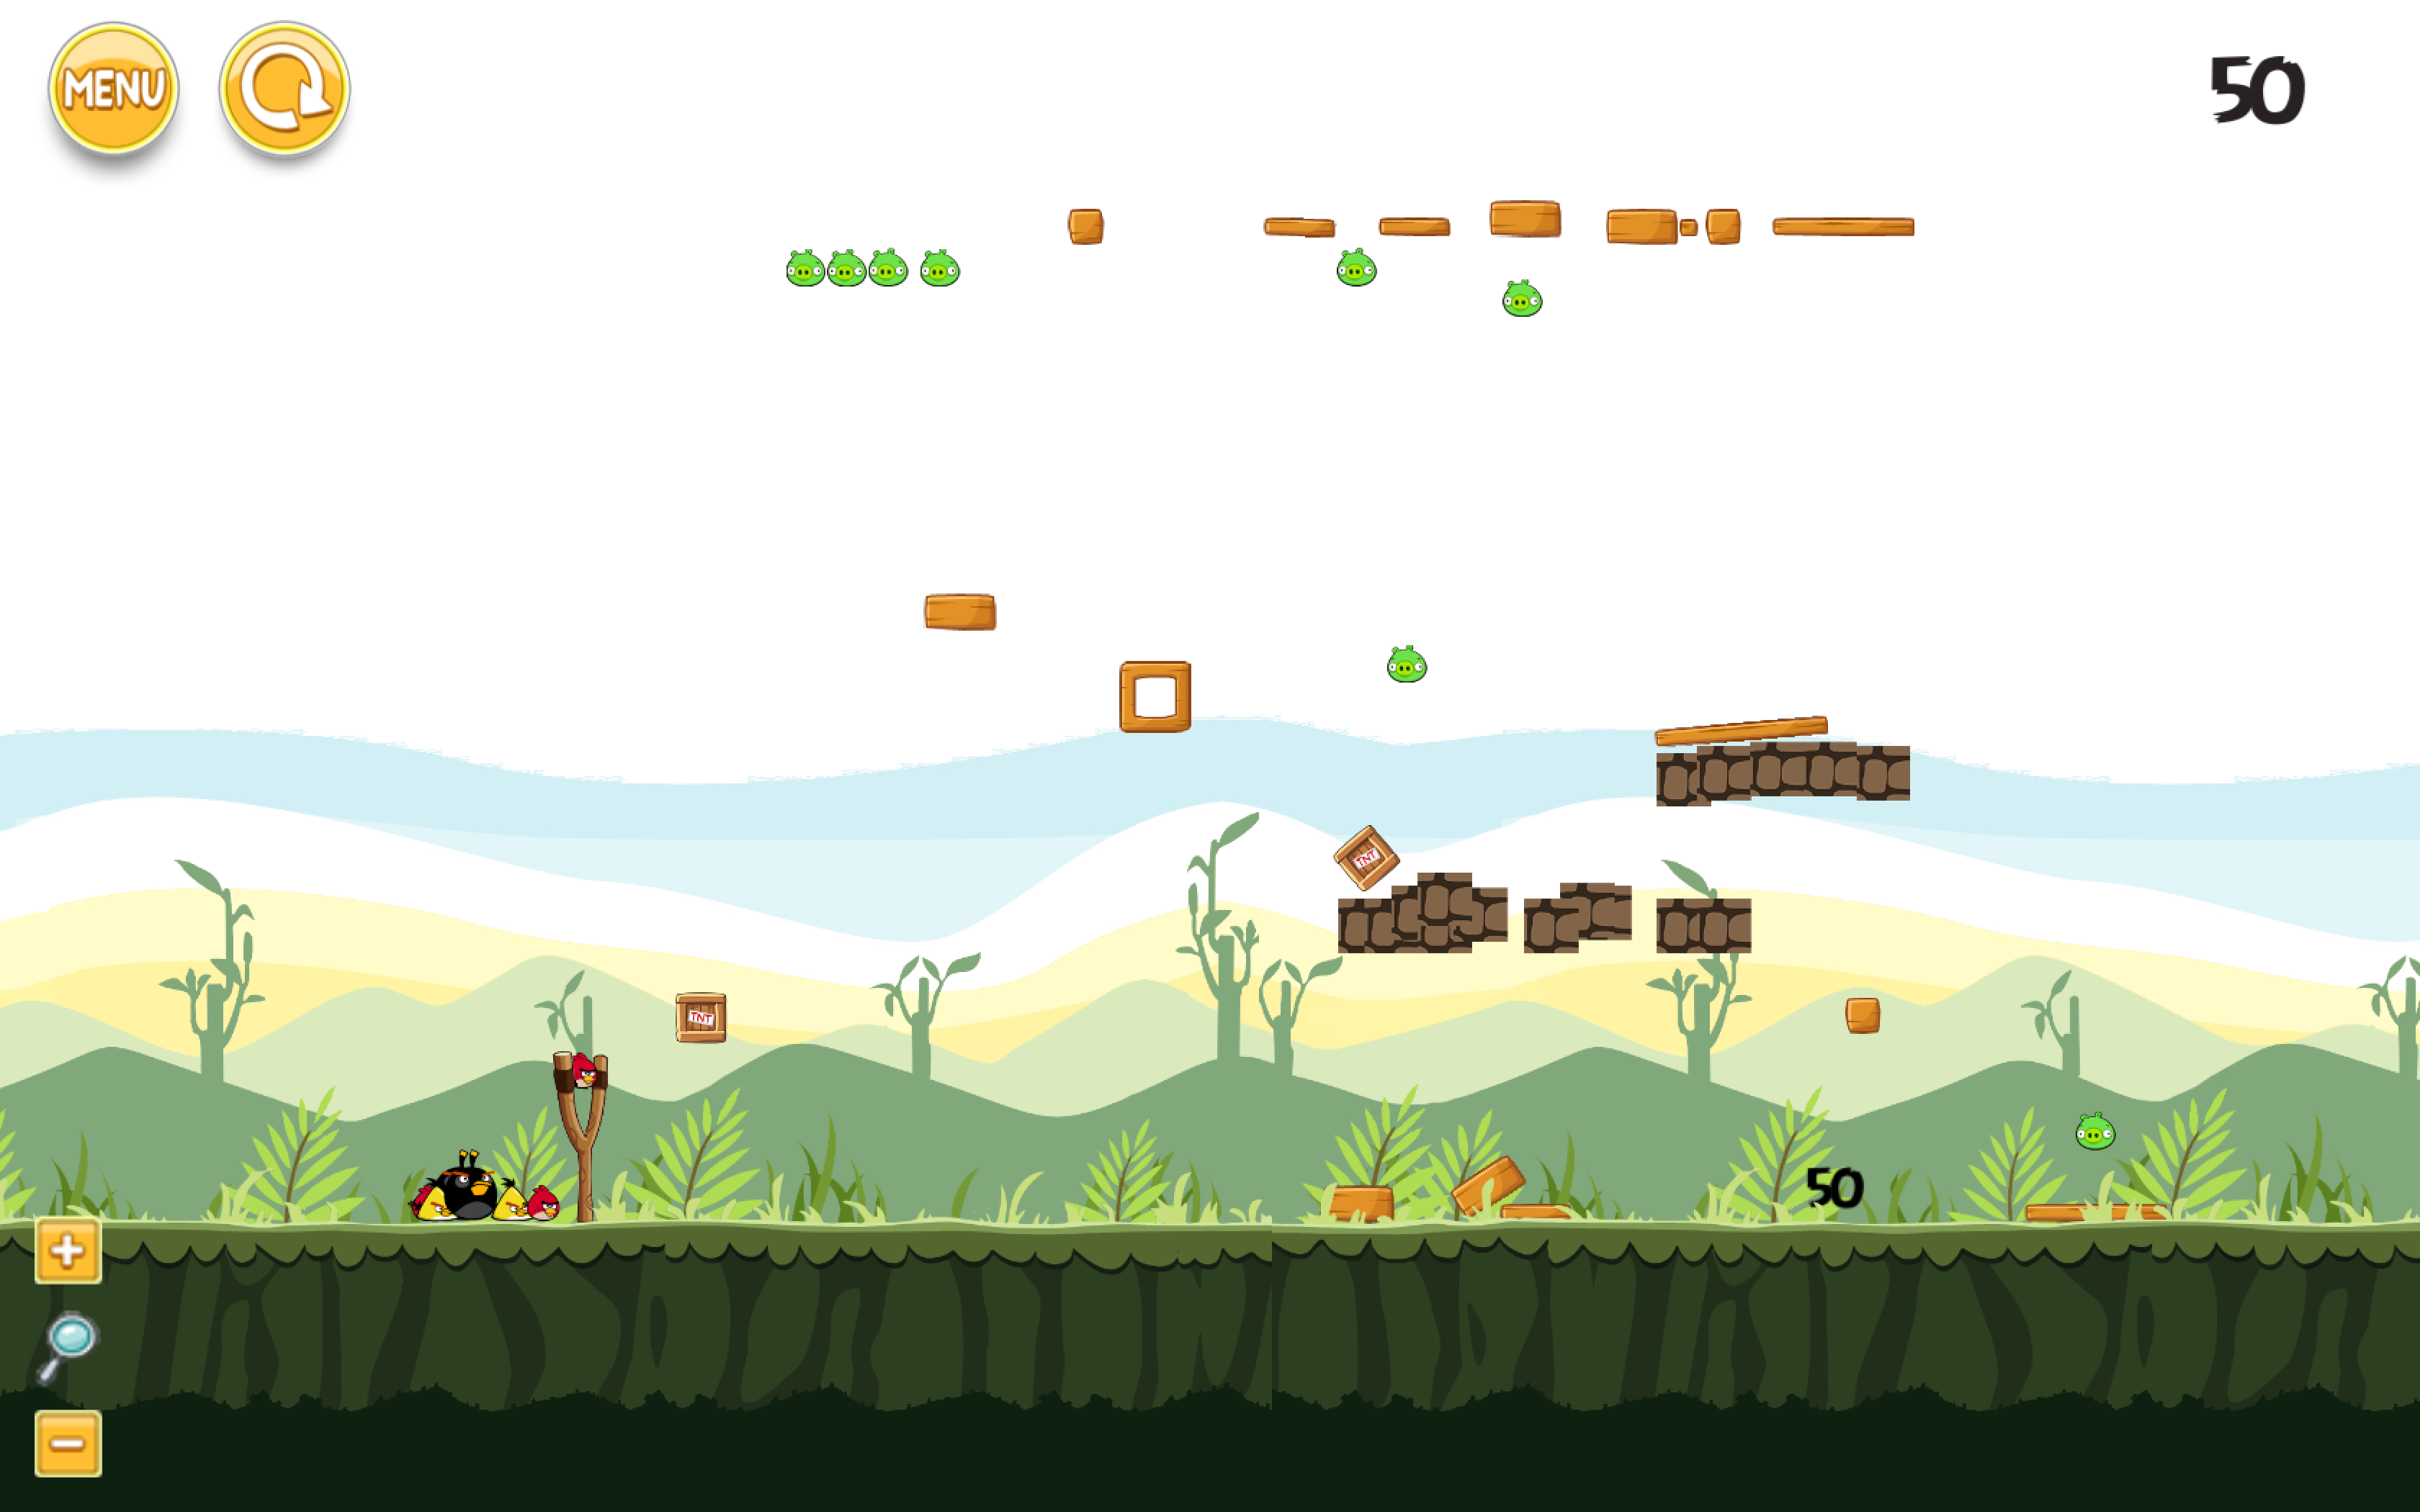
\includegraphics[height=12cm, width=17cm]{img/sample_level.png}
	\caption{Ergebnis eines durch Neuronale Netze generierten Levels}
\end{figure}
\section{Fazit}
Aus unseren Ergebnissen wird deutlich, dass GAN weniger zum Generieren von Level geeignet ist, da die erzeugten Level nicht sinnvoll sind. Das heißt, dass häufig obsolete Plattformen vorzufinden sind, welche in ihrem Aufbau und ihrer Struktur kein spielbares Level darstellen. Zudem erfolgt die Platzierung der Schweine und Hindernisse ohne jeglichen Wert auf Faktoren wie Spaß und Herausforderung zu legen, weswegen die generierten Level wenig für den Spieler bieten zu haben. Aufgrund dessen finden GANs ihren Einsatz oft nur bei der Erstellung photorealistischen Bildern zur Visualisierung verschiedener Gegenstände, bei der Modellierung von Bewegungsmustern in Videos, bei der Erstellung von 3D-Modellen von Objekten aus 2D-Bildern und bei der  Bildbearbeitung von astronomischen Bildern. Da unsere Methode der Neuronalen Netze keine brauchbaren Ergebnisse geliefert hat, wurde dieser beim Levelgenerator-Wettkampf nicht eingereicht. 
\section{Ausblick}
Für zukünftige Teams, die sich mit dem Projekt "AI Birds" des Lehrstuhls für Smart Environments befassen wollen, möchten wir als Abschluss Verbesserungsvorschläge des aktuellen Stands erläutern. Für die genannten Punkte bietet es sich an, den bereits vorhandenen Fortschritt zu verwenden und weiter auszubauen. Natürlich ist es aber auch möglich, komplett eigene Ansätze anzuwenden bzw. den vorhandenen Stand neu zu entwerfen. \\ Die Automatisierung der Abläufe funktioniert bereits einwandfrei und gemäß der Erwartungen. Trotzdem wäre es sinnvoll. eine GUI (z.B. mit JavaFX) zu entwerfen, um diesen Prozess überhaupt optisch darzustellen und dem Nutzer vor allem Übersicht über das Geschehen zu gewähren. Visuelles Feedback, was genau gerade passiert, wie weit der Automator vorangeschritten ist oder ob Fehler aufgetreten sind (mit genauem Fehlercode) sind sinnvolle Ergänzungen. \\ Eine weitere sinnvolle Ergänzung wäre die Umstellung auf Bordmittel, sodass so wenig wie möglich zusätzlich vom Nutzer installiert und angepasst werden muss. Der aktuelle Stand des Automators ist, dass der Code auf unser System zugeschnitten und zusätzlich Python, sowie der AutoSizer benötigt werden. Dies ist allerdings keine effiziente Lösung, weswegen eine Anpassung dem Nutzer ungemein helfen könnte. Dabei können externe Tools natürlich weiterhin installiert werden, die Installation davon sollte nur automatisch erfolgen.
[Verbesserungsvorschläge][Wie kann man GAN passend für Level-Generierung gestalten?] [RNN als mögliche Alternative?]
\subsection{GAN im Vergleich zu Alternativen}
Im direkten Vergleich von GAN mit den Alternativen empfiehlt es sich, die Meinungen und Erfahrungen von Experten heranzuziehen, die diese auch in der Praxis umgesetzt und angewendet haben, um so am effektivsten darüber urteilen zu können, wie GAN in Abhängigkeit seiner Alternativen abschneidet. [...]
\subsection{Weitere Tools als allgemeine Hilfestellung für das Projekt}
Im Laufe des Projekts war es gelegentlich der Fall, dass von uns entwickelte Tools für das Projekt obsolet wurden und wir diese letztlich nicht effektiv in unsere Aufgabenstellung miteinbringen konnten. Da diese aber trotzdem aufgebrachte Zeit für das Projekt in Anspruch genommen haben und sicherlich für zukünftige Teams von Vorteil sein könnten, möchten wir diese ebenfalls in diesem Abschnitt kurz erwähnen und in unsere Abgabe mit einfließen lassen. Einige dieser Tools sind bereits "ready-to-use", andere müssen jedoch ergänzt und weiter verfeinert werden.
\subsubsection{Doctor}
Dieses Tool wurde von Patrick Haller entwickelt und überprüft im eigenen System, ob die Umgebungsvariablen, welche für die Ausführung des Agenten und des Servers benötigt werden, existieren. Um den Doctor auszuführen steuert man in seinem Terminal das Verzeichnis other/doctor an und führt mit Python die \textit{doctor.py}-Datei aus (unter OS X aus dem Root-Verzeichnis: "\textit{cd ./other/doctor}" und führt den Befehl \textit{"python3 doctor.py"} aus). Das Tool überprüft nun, ob SWI-Prolog und die Nebenpakete von Python installiert sind. Die Version des Python-Interpreters wird ebenfalls überprüft, und falls diese nicht dem aktuellen Stand entspricht (Stand 24.09.2019: Python 3.7), erfolgt eine Aktualisierung.  Zudem muss der Java-Pfad ebenfalls ordnungsgemäß konfiguriert sein, weswegen der Doctor diesen in seine Checks miteinbezieht. Auf OS X kommt Homebrew bei der Installation zum Einsatz, unter Linux verwenden wir den Standard-Paketmanager und unter Windows haben wir uns für Chocolatey als Paketmanager entschieden. Auf Linux läuft dieser leider noch nicht einwandfrei, da manche Pakete nicht auf Linux zum Laufen gebracht werden konnten.
\subsubsection{JSON-XML-Parser}
Zur Generierung der Level war es notwendig, vorhandene Level, welche im JSON-Format codiert wurden, in äquivalente XML-Formate umzuwandeln. Dazu entwickelten wir einen XmlWriter sowie JsonToXmlParser in Python. \\ Der XmlWriter schreibt zunächst den standardisierten Kopf der XML-Dateien, welche die Codierung, die Breite des Levels (hier: 2) sowie die Minimum-/Maximum-Weite der Kamera beinhaltet. Der Parser liest nun die JSON-Datei und schreibt für jeden Block mithilfe der "add"-Methoden des XmlWriters die XML-Datei. Jeder eingelesene Vogel, Block, Schwein etc. wird dabei in seine eigene Liste eingeschrieben (inklusive der Attribute, z.B. "id", "rotation"...). Nach dem Erreichen des Endes der JSON-Datei erfolgt letztendlich der Abschluss des XML-Dokuments, bei welchem das Tag der GameObjects und vom Level geschlossen werden.